\paragraph{Methodology of the CALREC subproject.}

\begin{figure}
\begin{center}
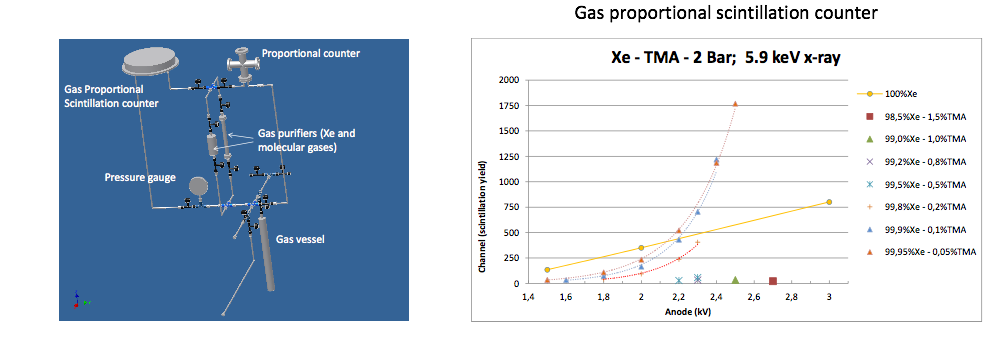
\includegraphics[width=0.99\textwidth]{img/TMA.png}
%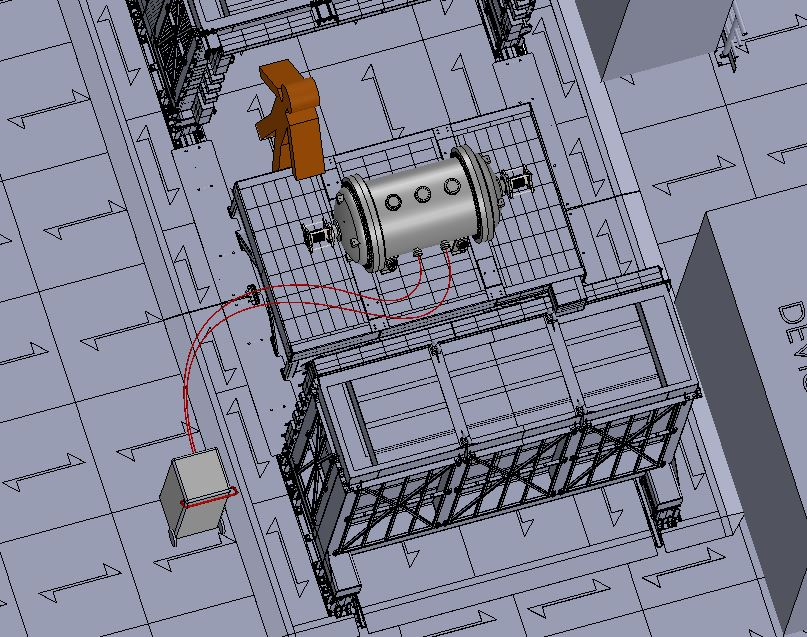
\includegraphics{img/CALIB_LSC_sources.jpg}
\caption{\small Left. A small experimental setup to test gas mixtures. Right: initial results obtained with the setup, showing that very small concentrations of TMA result in a very large increase of the scintillation yield. Larger concentrations, on the other hand, quench the yield. }
\label{fig:additives}
\end{center}
\end{figure}

The {\bf gain and noise of the PMTs and SiPMs sensors} will be calibrated using two sets of 400 nm LEDs located on the tracking and energy planes. The gain and noise of SiPMs and PMTs will be calculated for each sensor fitting their photo-electron response (e.g. the standard technique of estimating the gain from single photoelectron response). This procedure has been demonstrated in DEMO for the calibration of the energy plane\footcite{Lorca:2014sra}. In NEW, we will apply it also to the calibration of the last generation SiPMs deployed in the tracking plane, which have a much lower dark current than those deployed in DEMO (e.g., 100 kHZ per device to compare with several MHz) and are, therefore, capable of counting single electrons.

The CALREC subproject is also responsible for the {\bf energy calibration of the NEW and NEXT-100 detectors}. The energy scale and energy resolution has been measured in DEMO using \NA\ and \CS\ radioactive sources\footcite{Alvarez:2012nd,Alvarez:2013gxa}. A fit to the photoelectric spectrum of the gammas interacting in the gas yields a gaussian distribution whose mean value sets the energy scale, while the rms (or, as is customary in the field, the full width half maximum, FWHM) defines the resolution (see Figure \ref{fig.ERES}). In DEMO, the energy resolution has been measured at relatively low energies (550 and 660 keV), and the resolution in the region of \Qbb\ has been extrapolated using the scaling law $\delta E \propto 1/\sqrt{E}$, which has been demonstrated to hold well in the range between x-rays (35 keV) and \CS\ interactions (660 keV). 

The energy calibration in NEW and NEXT-100 will use the photo-peak of the 2.6 MeV gamma from a \Tl~  source to measure the energy resolution very near \Qbb. In addition, \NA\ and \CS~ sources will be used to calibrate the energy scale at  550 keV, 660 keV and 1.2 MeV. Adding the low energy point obtained with xenon X-rays (35 keV), we will be able to calibrate the energy in the full scale relevant for the experiment. The procedure is well understood from DEMO. The main novelty in NEW and NEXT-100 is the mechanical system, currently being designed, that allows us to introduce and withdraw the radioactive sources from the chamber, using special access ports. The calibration system will be built at US in the first 2 quarters of 2015 and installed at the LSC in Q3'15.

The \TL\ source also produces double electrons (double scape peak of \TL), with an energy of 1.6 MeV, not very far from \Qbb. Such double electrons, together with single electrons at 1.3 MeV from a \NA\ source can be used to measure single and double electron selection efficiency from the data themselves (recall that the selection of \bb\ events require a positive double-electron identification).

Calibration runs will be taken periodically. Typically a long run per month should be enough, but the exact procedure will be defined as part of the commissioning process of NEW and then of NEXT-100. 

The third objective of the CALREC subproject is the design, construction, commissioning and operation of a {\bf position calibration system}. Position calibration is needed to correct for the bias on the energy introduced by the geometry of the chamber. As demonstrated using NEXT-DEMO data\footcite{Lorca:2014sra} PMTs detect less light for events outside the central region of the detector. In DEMO, X-rays from \Xe ~ (35 keV) have been used to correct the position dependence of the energy. The procedure takes advantage of the fact that X-rays behave like point-like sources. One can, therefore, register their position in the detector (using the tracking plane) and measure their apparent energy (using the energy plane). The apparent energy differs from point to point, and thus one forms a weight matrix  (obtained normalising to the energy measured in the center of the camber) that is used to correct point-by-point the energy measured in the chamber.

Computing the energy weight matrix requires many X-rays interactions {\em in all the chamber}. In DEMO, those X-rays were produced by de-excitation of the gas when using conventional (\NA, \CS) radioactive sources. The statistics that can be collected with such a procedures is limited, however, and both NEW and NEXT-100 require much larger statistical samples.

We have proposed, therefore, the use of X-rays from Krypton, a technology demonstrated in liquid xenon detectors\footcite{Kastens:2009rt}. A source of $^{83}$Rb
decays to the metastable state  $^{83}$Kr$^m$~ with a half-life of 86.2 days. The
$^{83}$Kr$^m$~subsequently decays via emission of 3.1 keV and 9.4 keV conversion electrons with a half-life of 1.83 hours. Thus, no long-lived isotopes are introduced in the xenon gas, and the fact that krypton is itself a noble gas, guarantees no problems of chemical purity.  

The $^{83}$Rb~source is infused in a zeolite which is introduced in the gas system by adding a simple VCR cross (the zeolite itself is a small piece of 2 gram mass). The side arms of the the cross allow gas to flow through the chamber and a filter prevents the introduction of the zeolite into the gas system. The top arm of the cross allows the injection of the $^{83}$Rb~in the form of aqueous solution. A typical injection of 10 $\mu$l, discharged into the zeolite via a syringe yields 700 nCi of $^{83}$Rb. The rubidium itself stays attached to the zeolite, while the $^{83}$Kr$^m$~reaches an equilibrium rate in the range of several tens of kBq, enough to produce a very large statistical sample for calibration. Xenon is then circulated through the cross during several minutes, carrying the radioactive krypton gas with it.  

The rubidium source will be procured by the US group in 2015. The system will be commissioned in Q4'15 or Q1'16, depending of the progress of the energy-calibration system. Extensive analysis of rubidium data during 2016 will yield the weight matrix for NEW. The same procedure will be then repeated for NEXT-100. 

Finally, the ENG subproject will also be responsible for developing a dedicated testing system to evaluate {\bf additives capable to improve the performance of pure xenon}. The US will lead the R\&D focused in the studies of additives (for example TMA, tre-methylamine) mixed with xenon, which will be carried out in collaboration with the portuguese groups of Coimbra and Aveiro. These additives reduce the electron diffusion, which translate to a more confined trajectory.  In addition the scintillator light has  a 300 nm wavelength, easier to detect than the one of Xenon (170 nm). Furthermore, some of the additives (including TMA) are capable of transferring the charge from the Ba$^{++}$~ion produced in a \bb\ xenon decay to
the Ba$^{+}$~ion which can be tagged (e.g., $Ba^{++} + A \rightarrow Ba^{+} + A^{+}$) where $A$~is the additive. 

Figure \ref{fig:additives} (left) shows a small setup to measure the effect of additives in the gas. A preliminary result, using this setup shows that very small concentrations of TMA result in a very large increase of the scintillation yield. Larger concentrations, on the other hand, quench the yield. We plan a systematic campaign of measurements using several additives, (TMA, TEA,CH$_4$~CF$_4$~and others) that will study at depth the effect in yield, attachment and resolution of different mixtures (including very small concentrations) also as a function of pressure. This requires modification of the setup to allow operation at higher pressure, as well as monitoring systems to control very small concentrations of the additive. 

The initial R\&D will be done with the simple setup already available, at pressures of up to 2-3 bar. During 2015, we will characterise different additives and choose the most suitable ones for NEXT. In 2016, the setup will be upgraded to take higher pressures and further studies will be performed up to operating pressures of 10-15 bar. In 2017 we plan to operate the DEMO detector with the chosen additive, to characterise the performance of the mixture in a large system. We will use our calibration protocol, describe above, to measure electron tracks and energy resolution at different energies, to quantify the potential improvements of the mixture. 

In addition, we will carry an experiment, in coordination with the \BATA\ program  to measure the charge transfer $Ba^{++} + A \rightarrow Ba^{+} + A^{+}$, where $A$~is the chosen additive. The exact schedule of such an experiment will depend on the overall \BATA\ program, but we expect that it will be performed in 2016.